
\section{Additional Results} \label{AppendixA}

\subsection{Logistic regression for assistance applications}


\begin{table}[htbp]
   \centering
   \caption{\label{ResultsLogit} Determinants of Assistance Application}
   \begin{tabular}{lc}
      \tabularnewline\midrule\midrule
      Dependent Variable:        & Applicant\\
      Model:                     & (1)\\
      \midrule \emph{Variables} &  \\
      (Intercept)                & -3.622\\
                                 & (3.723)\\
      Share of democratic voters & -0.8362$^{**}$\\
                                 & (0.3469)\\
      Median Income (logs)       & 0.2939\\
                                 & (0.3331)\\
      Poverty Rate               & 4.033$^{**}$\\
                                 & (1.575)\\
      Share of single mothers    & 4.068$^{***}$\\
                                 & (1.144)\\
      \midrule \emph{Fit statistics} &  \\
      Observations               & 2,882\\
      Squared Correlation        & 0.02306\\
      Pseudo R$^2$               & 0.01966\\
      BIC                        & 3,724.7\\
      \midrule\midrule\multicolumn{2}{l}{\emph{IID standard-errors in parentheses}}\\
      \multicolumn{2}{l}{\emph{Signif. Codes: ***: 0.01, **: 0.05, *: 0.1}}\\
   \end{tabular}
\end{table}





\section{Pre-Treatment Trends} \label{PreTrends}

Here we display plots of aggregated pre-treatment trends to justify the parallel trends assumption. Mean test scores are aggregated by cohort (year of first treatment) and relative time to treatment, and never treated units act as the control group. Figure \ref{PreTrendsMath} and \ref{PreTrendsRLA} show the results for mathematics and RLA respectively. We only display these plots for overall test scores and not for subgroups. However, the plots for the subgroups look very similar.


\begin{figure}[!h]
	\centering
	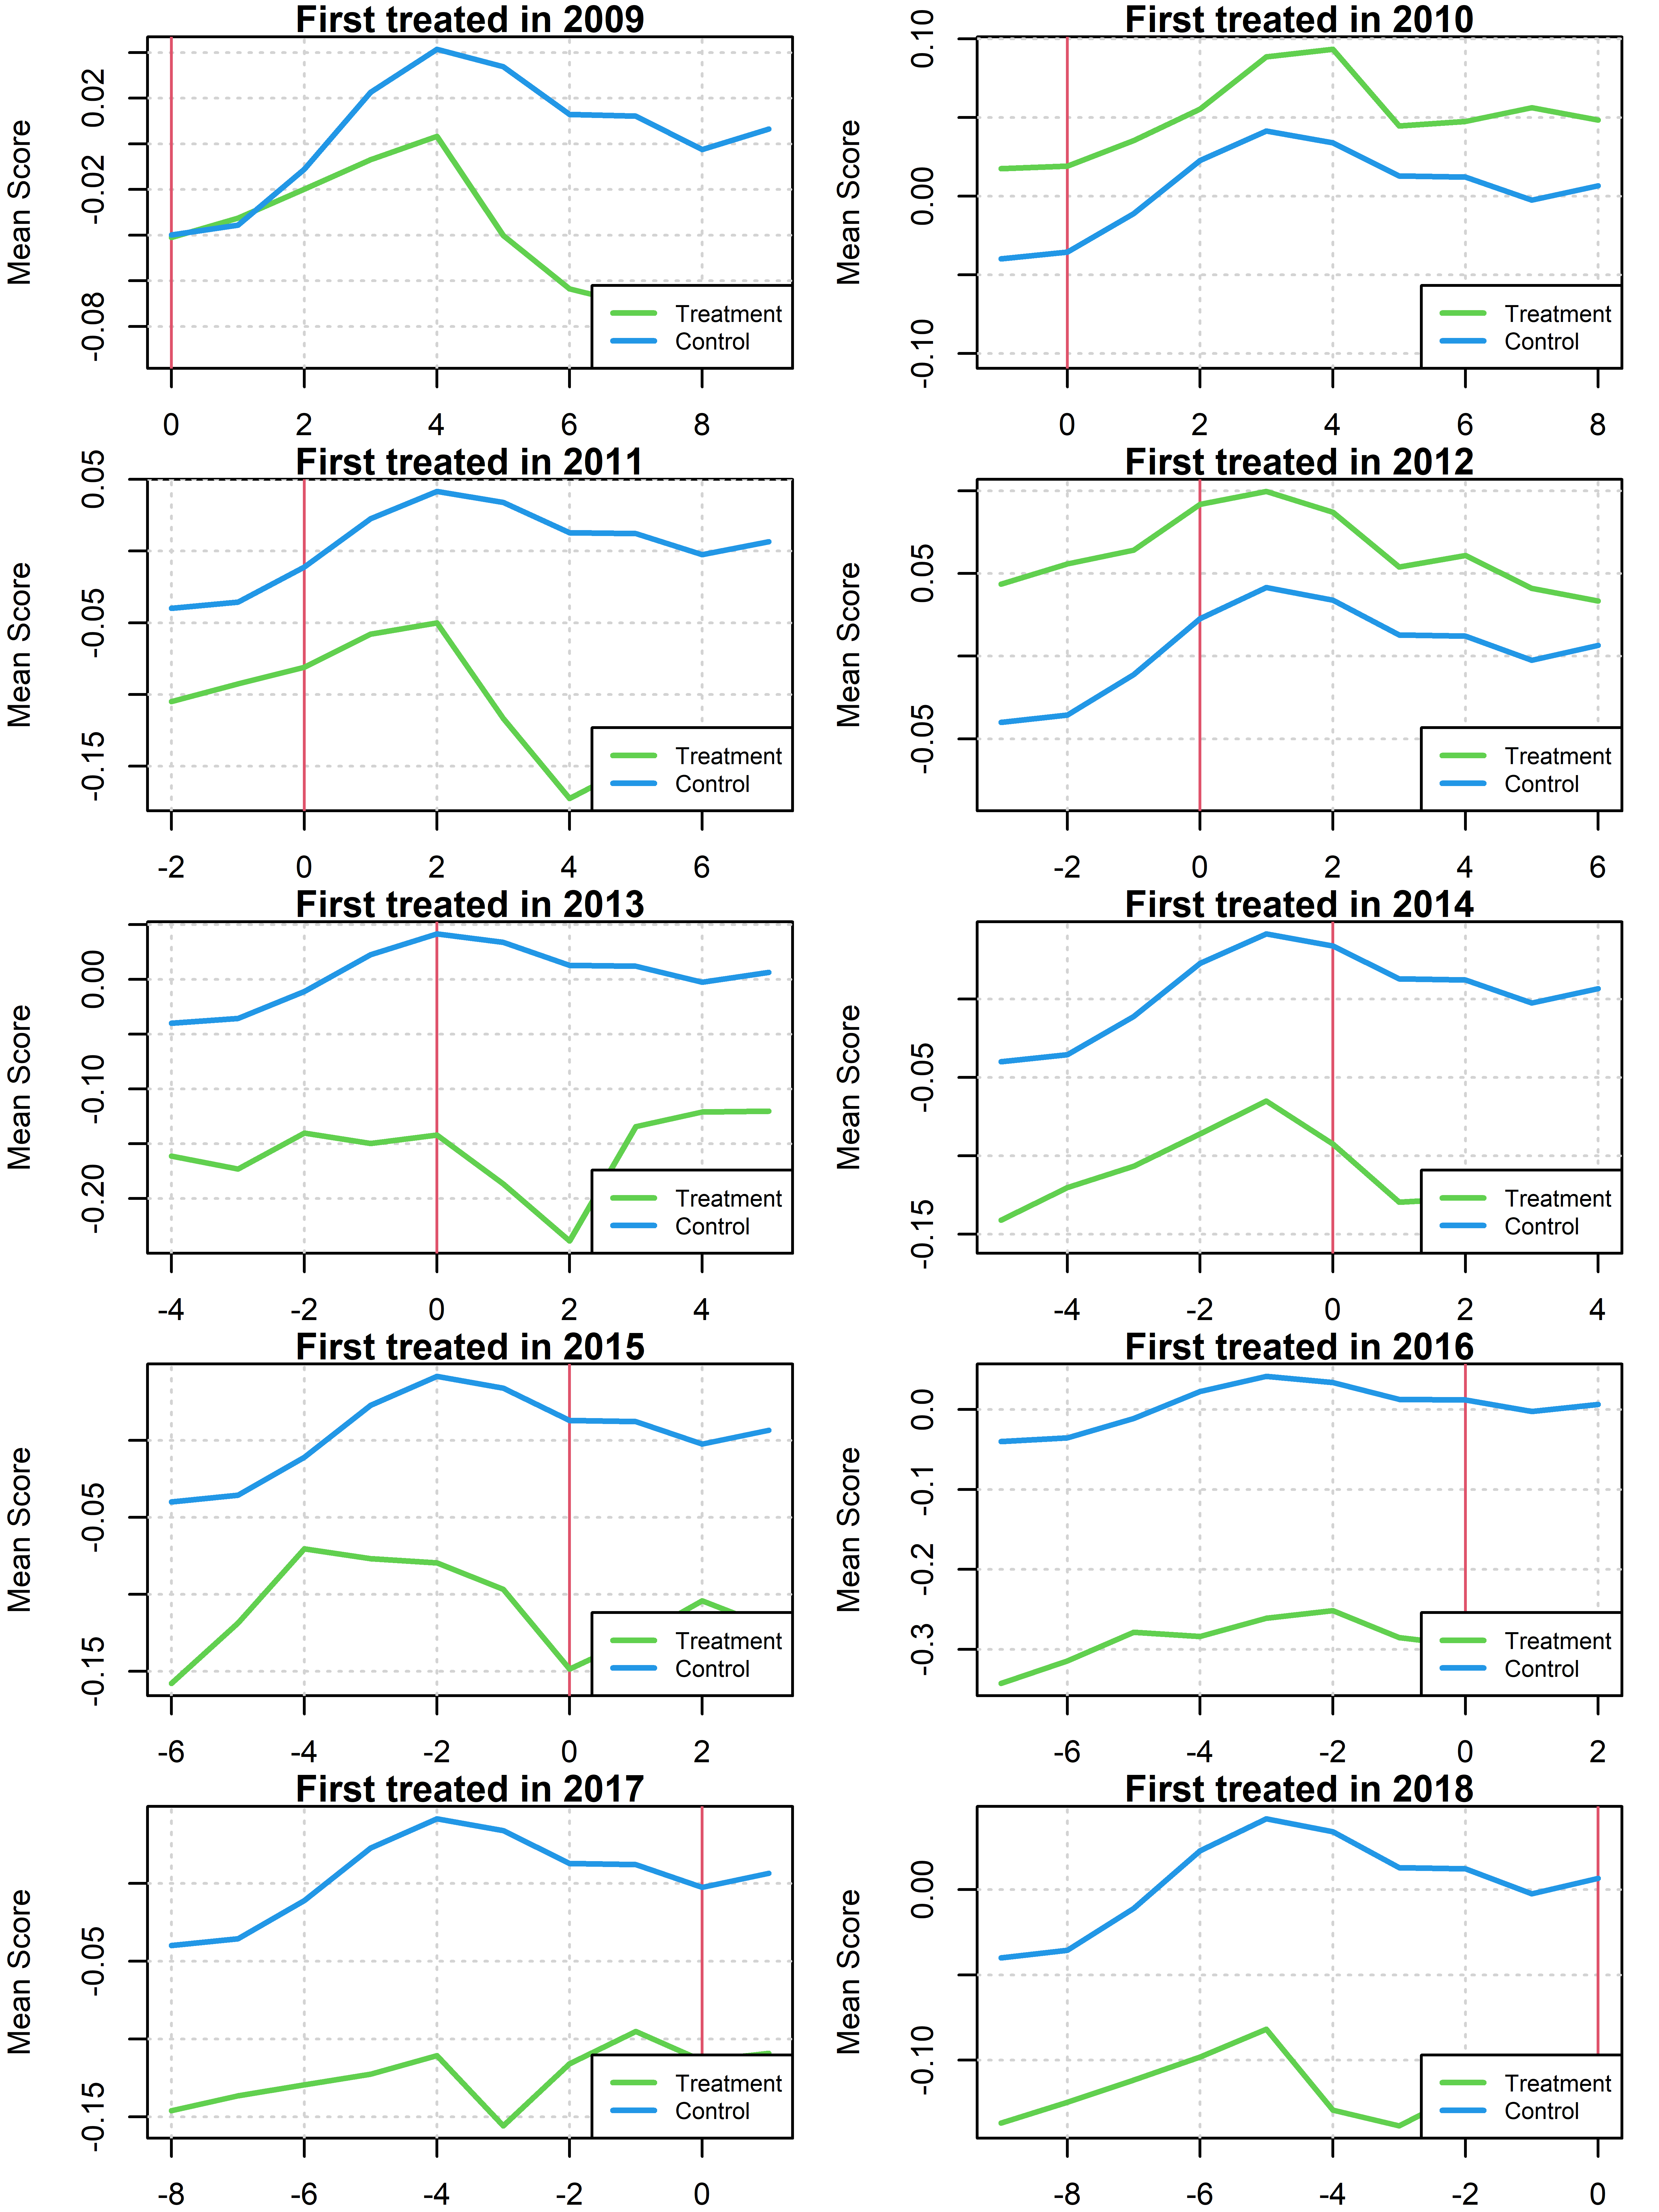
\includegraphics[scale=1]{"../Code & Data/ParTrendsPlotMathematics.png"}
	\caption{Pre trends for aggregated mean scores in mathematics}
	\label{PreTrendsMath}
\end{figure}

\begin{figure}[!h]
	\centering
	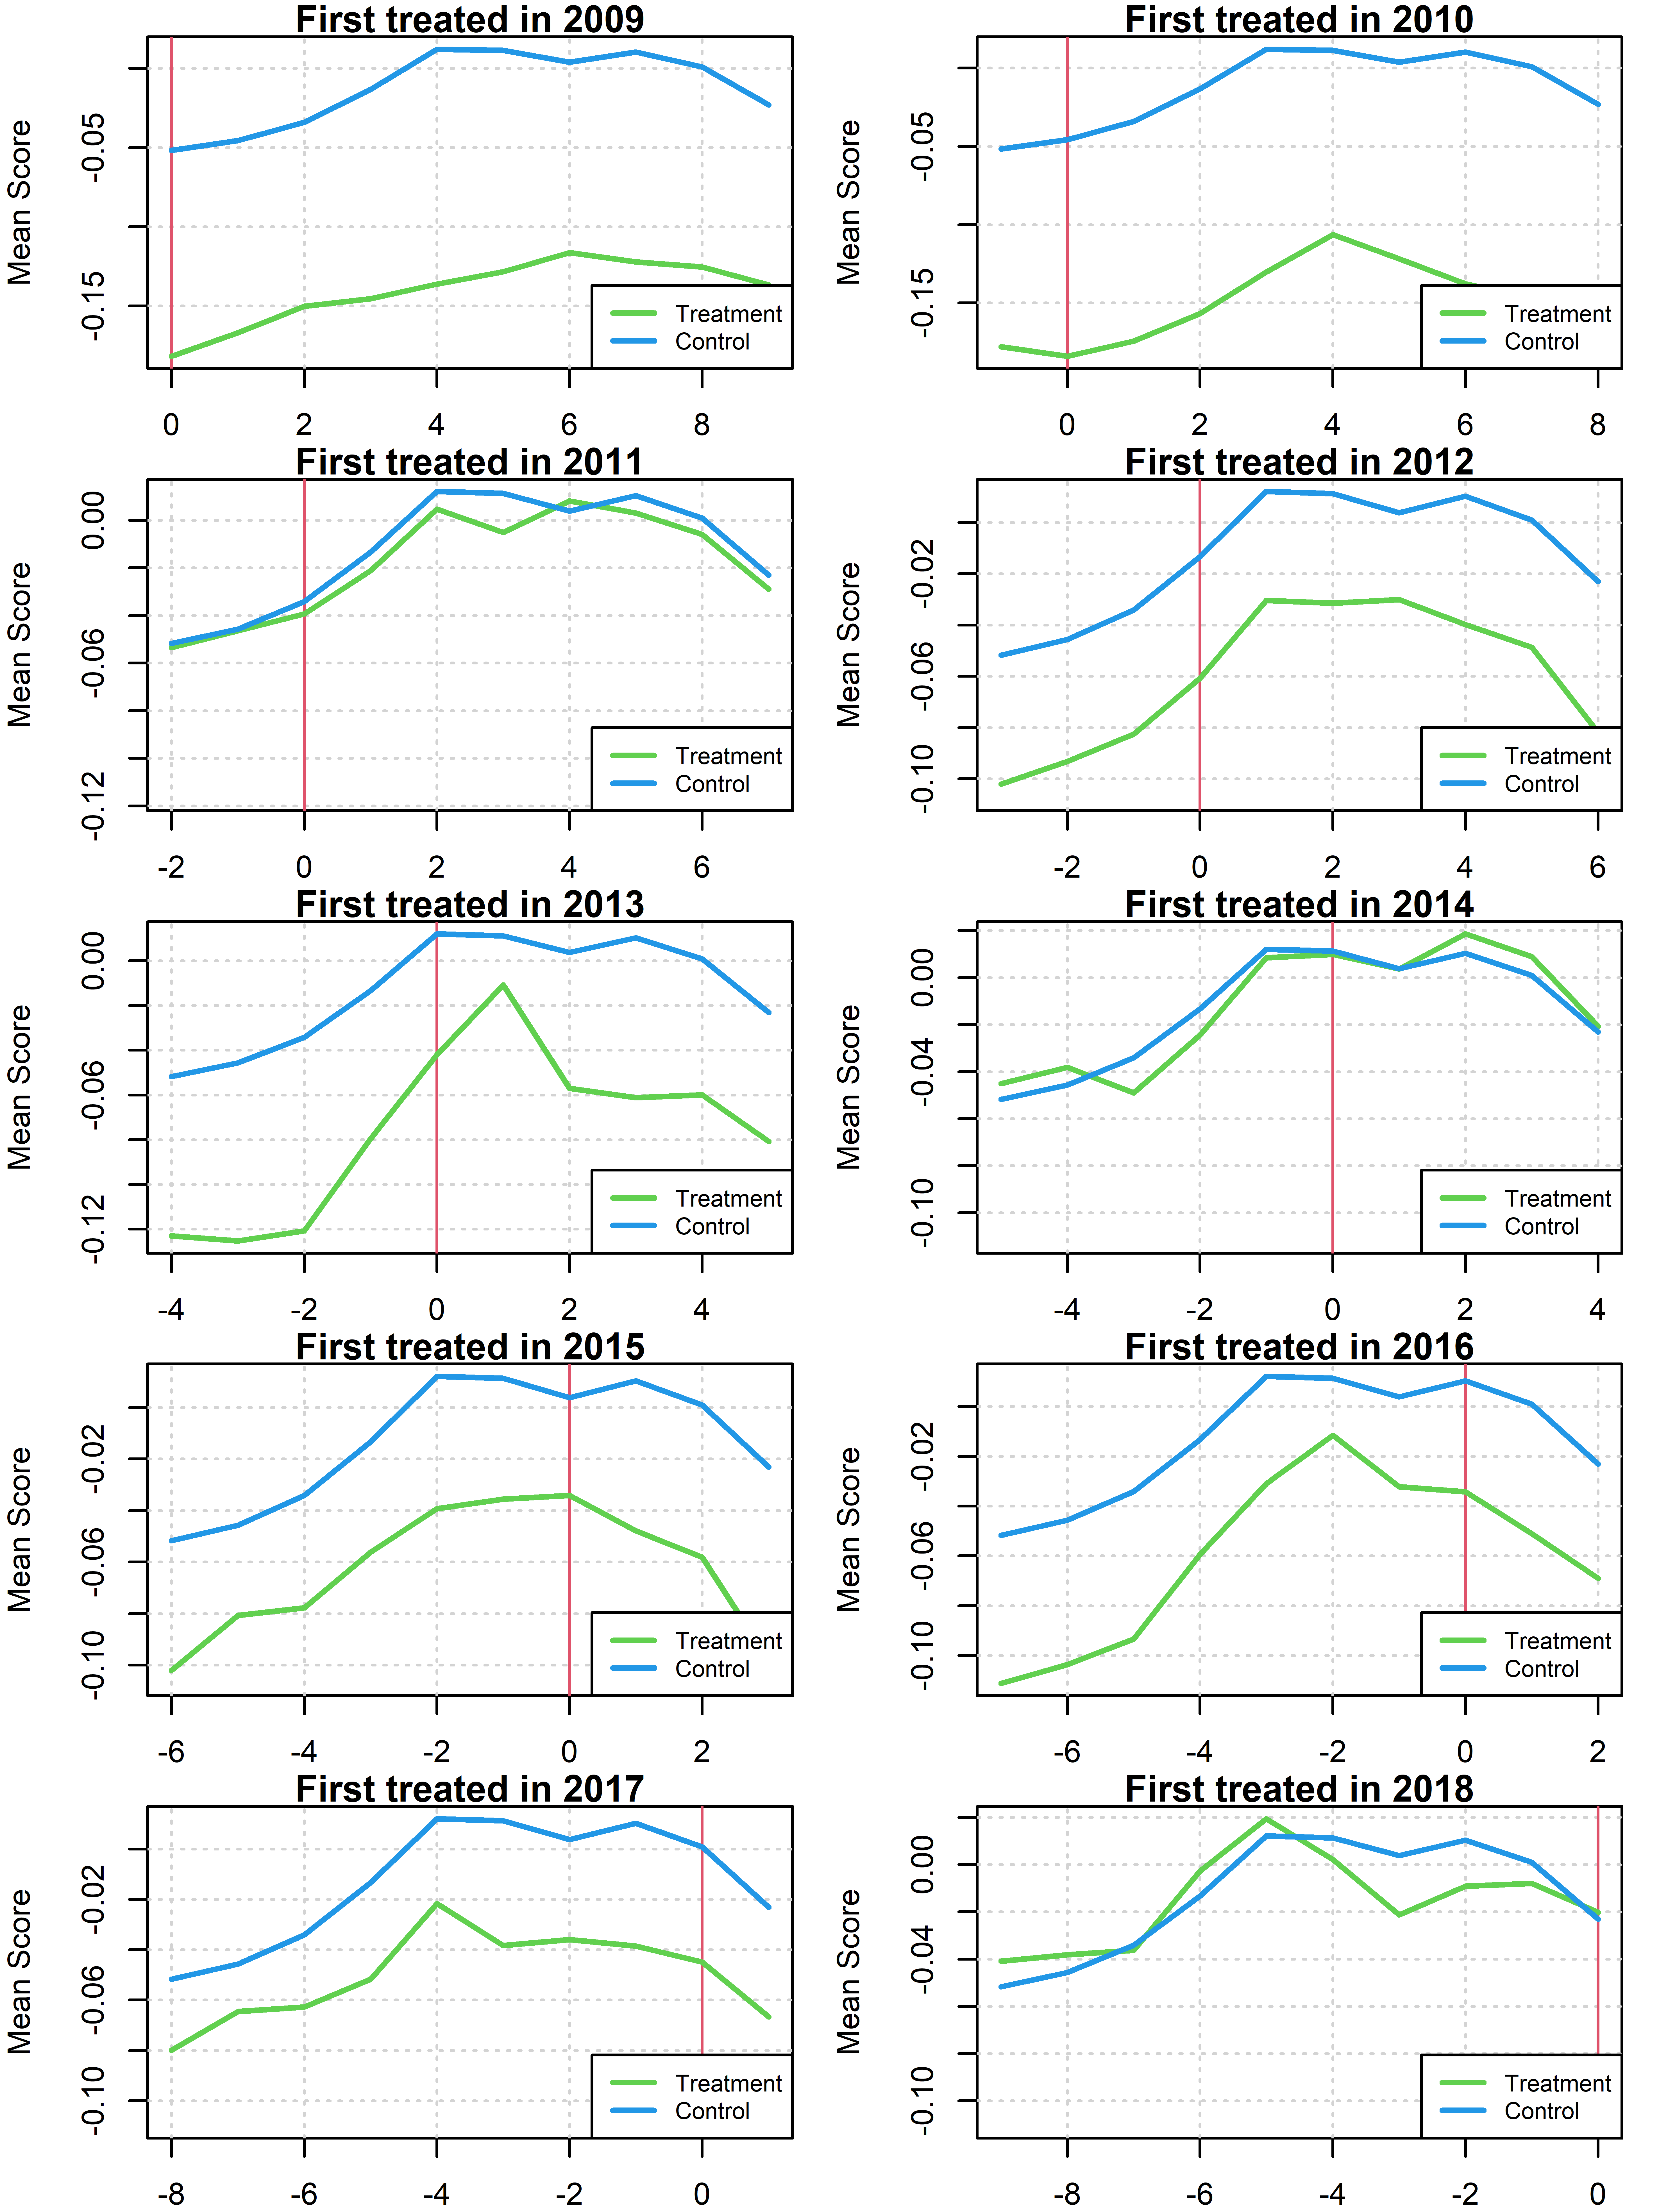
\includegraphics[scale=1]{"../Code & Data/ParTrendsPlotRLA.png"}
	\caption{Pre trends for aggregated mean scores in RLA}
	\label{PreTrendsRLA}
\end{figure}



